\section{Introduction}

The \textit{proceedings} are the records of a conference.\footnote{This
  is a footnote}  ACM seeks
to give these conference by-products a uniform, high-quality
appearance.  To do this, ACM has some rigid requirements for the
format of the proceedings documents: there is a specified format
(balanced double columns), a specified set of fonts (Arial or
Helvetica and Times Roman) in certain specified sizes, a specified
live area, centered on the page, specified size of margins, specified
column width and gutter size.

\begin{figure*}[t]
	\centering
	\begin{minipage}{0.39\textwidth}
		\centering
		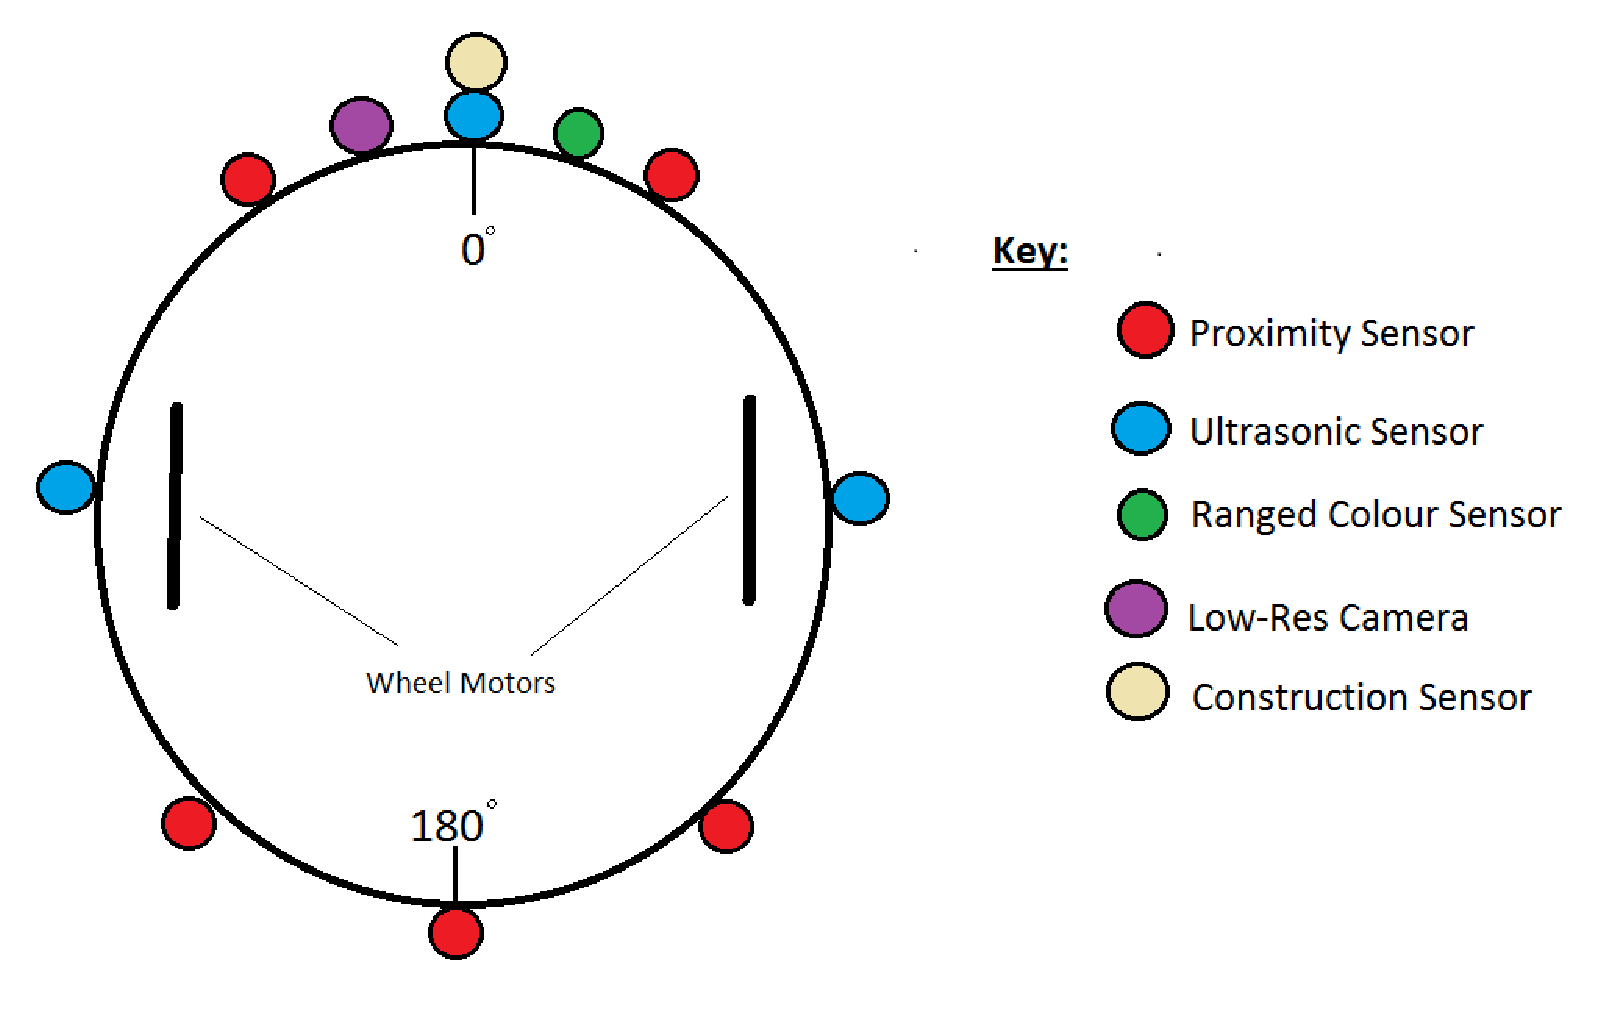
\includegraphics[width=\textwidth]{Morphology.eps}
	\end{minipage}
	\centering
	\begin{minipage}{0.60\textwidth}
		\centering
		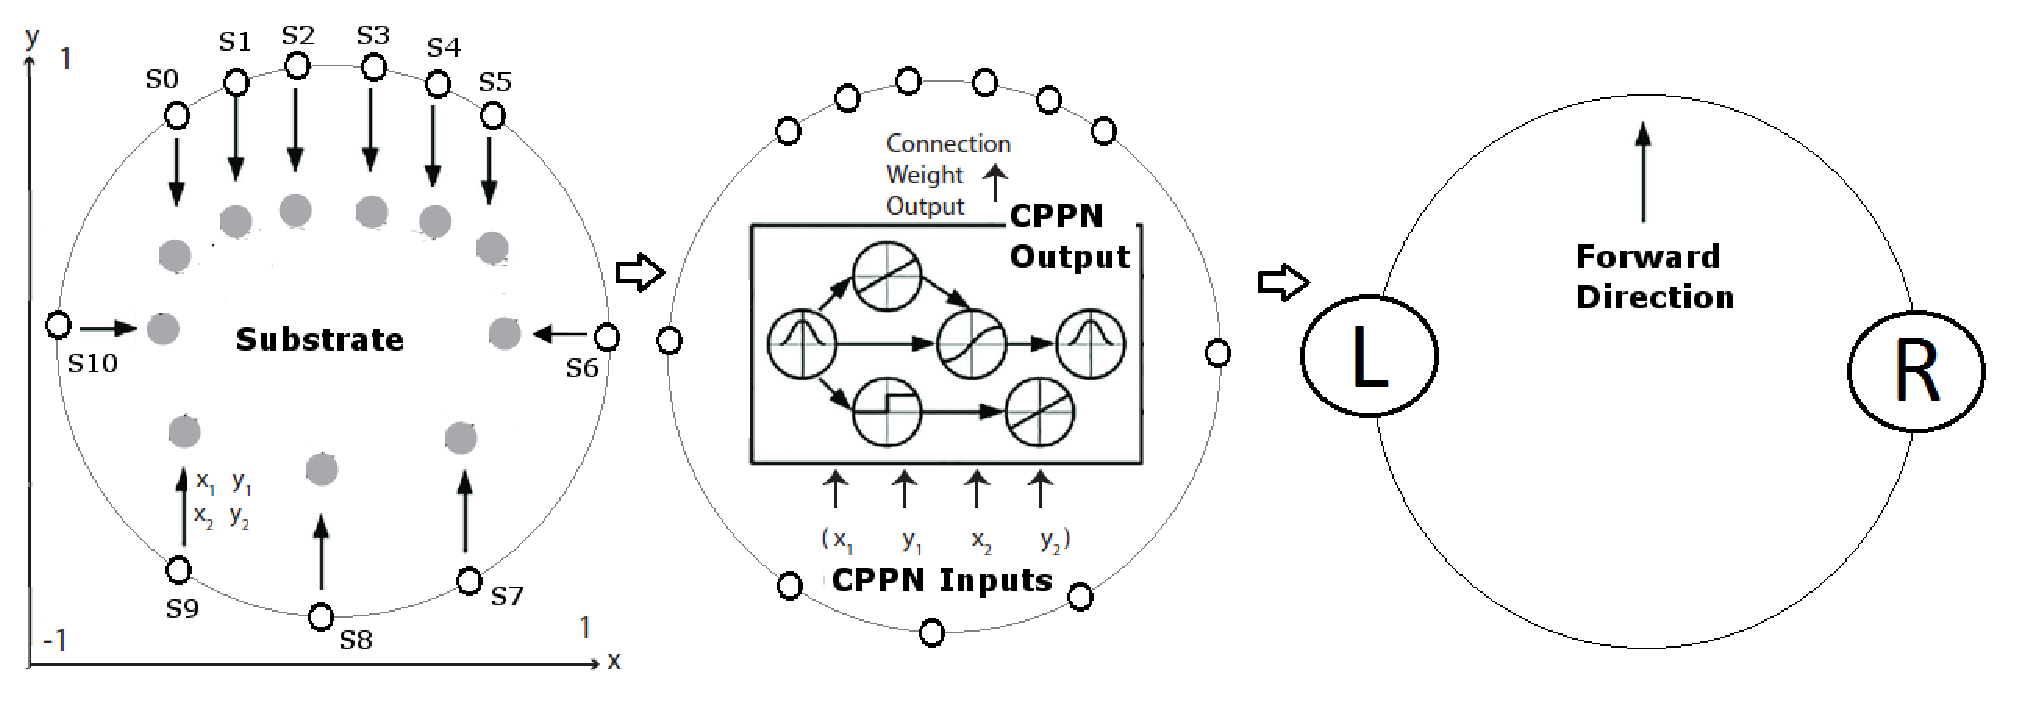
\includegraphics[width=\textwidth]{ANN_Config3.eps}
	\end{minipage}
	\caption{\textit{Left (color):} Robot morphology $1$, with relative positions of various sensors on the robot.
		\textit{Right (gray-scale):} ANN Topology as it relates to robot morphology $1$: $11$ Sensory inputs [S0, S10].  Sensory inputs connect to a hidden
		layer (left).  Connection weight values between two nodes ($x_{1}$, $y_{1}$, $x_{2}$, $y_{2}$) are evolved by querying the CPPN (center) with x, y
		values in the range [-1, 1] (axis shown).  The hidden layer is fully connected to all inputs and outputs (connectivity not depicted).
		Motor outputs (right)
		\textit{L} and \textit{R} determine the speed of the left and right wheels, respectively, and thus a robot's speed and direction.}\label{fig:ann}
\end{figure*}

\section{Methods}

HyperNEAT \cite{StanleyDAmbrosioGauci2009} is an extension of NEAT (\textit{Neuro-Evolution of Augmented Topologies})
\cite{StanleyMiikkulainen2002}, where ANNs are indirectly encoded using a CPPN (\textit{Compositional Pattern Producing Network})
\cite{Stanley2007}.
HyperNEAT was selected as it has a number of benefits demonstrated in previous work \cite{DAmbrosio2013},
\cite{WatsonNitschke2015SSCI}.
This includes its capability to exploit geometric features such as symmetry, regularity and modularity
in robot morphology and the task environment during controller evolution.
%in the  geometric features include the relative positions of other robots, blocks,
%the direction robots and blocks are facing and the shape of the environment.
%Also, the structures to be built are modular
%(comprised of blocks) and often regular (the same sequence of blocks can be repeated).

In this study, HyperNEAT evolves the connection weights between each robot's sensory input layer,
hidden layer and motor output layer, where each robot used the same controller, making teams
homogenous.
Controller evolution experiments were initialized with a given morphology (table \ref{tab:morphConfigs}).
\hl{However, in one experiment set, each robot's sensor configuration of team morphology could be
\textit{co-adapted} via HyperNEAT activating and deactivating sensory input node connections over
the evolutionary process. THIS CAN BE REMOVED?}
For these experiments (section \ref{sec:experiments}), \textit{add connection} and
\textit{remove connection} mutation operators (table \ref{tab:simParameters}) from previous work
\cite{HewlandNitschke2015} were applied every generation to a sensory input node
chosen with uniform random selection.  \hl{The mutation operator applied depended on whether the chosen input
node was connected or not. DOES THIS STILL REFER TO THE WHOLE APPROACH OF RANDOMLY ACTIVATING OR DEACTIVATING}  The construction zone sensor (table \ref{tab:morphConfigs}) was permanently activated
for all morphologies and could not be disconnected, as this enabled robots to detect \textit{construction zones}
(section \ref{subsec:constructionTask}).

Table \ref{tab:morphConfigs} presents a list of \textit{morphology identification} (ID) numbers and the
number and type of sensors that correspond to each morphology.
\hl{For example, morphology 2 has four proximity sensors, one ultrasonic sensor, one colour-ranged sensor, and
one low-resolution camera. FIND ANOTHER EXAMPLE TO USE HERE USING THE NEW MORPHOLOGIES}.
Note that all morphologies have a construction sensor as this is necessary to complete the collective construction task.

%\vspace{-0.4cm}
\subsection{Robot Team Controller}\label{sec:embodiment}
%\vspace{-0.2cm}
Each robot in the team used an ANN controller with
\textit{N} sensory input nodes, determined by the given morphology being evaluated (table \ref{tab:morphConfigs}).
Each robot's controller mapped sensory inputs, via a fully connected hidden layer, to two motor outputs, the
robot's left and right wheels (figure \ref{fig:ann}). %using HyperNEAT \cite{StanleyDAmbrosioGauci2009}.

Figure \ref{fig:ann} illustrates the sensory configuration for \textit{N} = $11$ (morphology $1$), and the
associated substrate and CPPN used by HyperNEAT.
For each robot morphology (table \ref{tab:morphConfigs}), the sensors corresponding to the input layer
of the controller was a circle \textit{N} nodes distributed about a robot's periphery,
where the exact geometric configuration corresponded to the morphology being evaluated
(figure \ref{fig:ann} illustrates morphology
$1$)\footnote{Illustrations of all robot morphologies tested can be found at: \url{https://github.com/not-my-name/SSCI_Paper_Appendix}}.
The intermediate ANN hidden layer reflects the configuration of the input layer, preserving
the geometry of the sensory input layer, that is, the direction of each sensor's FOV (figure
\ref{fig:ann}). \hl{THIS IS WHERE THE FOOTNOTE WITH THE LINK TO THE ILLUSTRATIONS ON GITHUB IS. REMEMBER TO CHANGE TO THE NEW REPO}
The ANN was initialized with random weights normalized to the range [-1.0, 1.0], with full connectivity between adjacent layers,
however, partial connectivity was evolvable via the CPPN generating a zero weight.
Collectively all sensors approximated up to a $360$ degree \textit{Field of View} (FOV).

The nodes comprising each robot's ANN controller, connected by the CPPN, were placed in the substrate
illustrated in figure \ref{fig:ann}.
Each node in the substrate was placed at specific ($x$, $y$) locations in the two-dimensional geometric space
of the substrate ($x$, $y$ axes were in the range: [-1, 1]).
Connection weights in the controller were evolved via querying the CPPN for the weight of any connection
between two points ($x_{1}$, $y_{1}$) and ($x_{2}$, $y_{2}$) by inputting ($x_{1}$, $y_{1}$, $x_{2}$, $y_{2}$)
into the CPPN, which subsequently output the associated weight.
During HyperNEAT's evolutionary process, the CPPN was evolved via having nodes and connections added and removed, as well
as connection weight values mutated \cite{StanleyDAmbrosioGauci2009}.

Thus, the CPPN evolved a connectivity pattern across the geometry of the ANN via querying all the potential
connections for their weights.
This connectivity pattern was effectively a function of the task and ANN geometry,
which enabled HyperNEAT to exploit the structure (regularity, repetition and symmetry) of the task and robot morphology.
For example, there was symmetry in the robot morphology in terms of the positioning of sensors about each
robot's periphery (figure \ref{fig:ann}) and there was regularity and repetition in the collective construction
task, in terms of repeating block types comprising modular and regular structures.
In the collective construction task, \textit{modularity} was defined as the composition of modular structures
(buildings in construction zones) from a sequence of connected blocks and \textit{regularity} was defined
as the same sequence of blocks repeated in a building.

Previous work has demonstrated that the indirect encoding of an evolved CPPN facilitates the evolution of
robot controllers with increased task performance enabled by a compact representation
of task and robot geometry \cite{DAmbrosioStanley2008}, \cite{WatsonNitschke2015SSCI}.
Table \ref{tab:simParameters} presents the HyperNEAT parameters used in this study, where \textit{delta}
was angle between the ($x_{1}$, $y_{1}$, $x_{2}$, $y_{2}$) positions of nodes in the substrate.
These parameter values were determined experimentally.   All other HyperNEAT parameters not listed in
table \ref{tab:simParameters}, were set as in previous work \cite{DAmbrosioStanley2008}.
%The ANN uses a three dimensional coordinate system for processing \textit{x}, \textit{y}, \textit{z}
%positions in the CPPN in order to generate weight and bias values and connectivity.
%Previous work  also demonstrated that HyperNEAT exploits the sensory-motor node configuration in ANN controllers,
%Nodes for processing sensory inputs correspond to the direction each sensor faces.

\subsubsection{Detection Sensors}
Each robot was equipped with various sensor types, where the exact sensor complement, including the
relative position and direction on the robot depends upon the given experiment
(section \ref{sec:experiments}) and morphology being evaluated (table \ref{tab:morphConfigs}).
Each robot had \textit{N} sensors corresponding to the \textit{N} inputs comprising the robot's
ANN sensory input layer (figure \ref{fig:ann}), each with a range of \textit{r}
(portion of the environment's length).
A robot's sensory FOV was split into \textit{N} sensor quadrants, where all sensors were constantly active
for the duration of the robot's lifetime.
The \textit{nth} sensor returned a value in the normalized range [0.0, 1.0],
in the corresponding \textit{nth} sensor quadrant.
A value of $0.0$ indicated that no blocks were detected and a value of $1.0$ indicated that an object was detected
at the closest possible distance to the given sensor.
%All detection sensor values are

Table \ref{tab:simParameters} presents the different sensor types used in this study, where the functional properties of each sensor
(range and FOV) were abstractions of corresponding physical sensors typically used on the Khepera III robots \cite{khepera3usermanual2013}.
In table \ref{tab:simParameters}, range values are units defined in relation to the environment size ($20$ x $20$)
and FOV values are in radians.
Each morphology also included a special construction zone detection sensor that activated with a value in the range
[0.0, 1.0] whenever a robot came into
contact with a block that must be connected with other already connected blocks.

The construction zone sensor calculated the squared Euclidean norm, bounded by a minimum observation distance, as an
inversely proportional distance between \textit{this} robot and the closest construction zone, where a value of 1.0 indicated the robot (pushing a block)
was in contact with the construction zone and a value of 0.0 indicated that the robot (pushing a block) was the maximum possible
distance from the closest construction zone.
Robots were unable to detect each other, thus all cooperative interactions were \textit{stigmergic} \cite{BeckersHollandDeneubourg1994}
where robots interacted via pushing blocks into the environment's construction zone.
\hl{Furthermore, robots had no \textit{a priori} knowledge of the construction schema,
but rather must discover the construction schema rules by trial and error.NOT USING A CONSTRUCTION SCHEMA ANYMMORE. MENTION HERE THAT IT ONLY REQUIRES COOPERATION??}
Also, once at least two blocks had been pushed and connected together this formed a construction zone (section \ref{subsec:constructionTask}),
that was then visible to each robot's construction zone sensor.
%Each robot has \textit{N} sensors each with a specified range, field of view and bearing (its position on the robot). The subject of these experimental comparisons is the various combinations of these different types of sensors (referred to as sensor morphologies) that are implemented in the different experiments. These sensor morphologies are predetermined by the experimenter and are outlined later on in this table. Robots are unable to detect each other, thus all cooperative interactions are \textit{stigmergic} \cite{BeckersHollandDeneubourg1994}

\begin{table*} [t]
	\renewcommand{\arraystretch}{1.50}
	\caption{Sensory configuration (number of sensors) for each morphology.}\label{tab:morphConfigs}
	\centering
	\begin{tabular}{| c | c | c | c | c | c |}
		\hline
		\textbf{Morphology ID} & \textbf{Proximity Sensors} & \textbf{Ultrasonic Sensors} & \textbf{Color Ranged Sensors} & \textbf{Low-Resolution Camera} & 	 \textbf{Construction Zone Sensors} \\
		%                       &   Sensors     &   Sensors          &  Sensors         &   Camera          &   Zone Sensors \\
		\hline
		\textbf{1}               &	5 	 	    & 	3  	             &	1               &	1                &	1   \\
		\textbf{2}               &	3 	 	    &	2		         &	1	            &	1                &	1   \\
		\textbf{3}               &	1	        &	0				 &	1			    &	1                &	1    \\
		\hline
	\end{tabular}
\end{table*}


\subsubsection{Movement Actuators}

Two wheel motors control a robot's heading at constant speed.
Movement is calculated in terms of real valued vectors (\textit{dx}
and \textit{dy}).  Wheel motors (\textit{L} and \textit{R} in figure \ref{fig:ann})
need to be explicitly activated.
A robot's heading is determined by normalizing and scaling its motor
output values by the maximum distance a robot can traverse in one
iteration (table \ref{tab:simParameters}).  That is:

%\begin{equation}\label{equ:contDisCalc}
$\textit{dx} = d_{max} (o_{1} - 0.5)$

$\textit{dy} = d_{max} (o_{2} - 0.5)$
%\end{equation}

Where, $o_{1}$ and $o_{2}$ are the motor output values, corresponding
to the left and right wheels, respectively, producing an output in the range:
[-1.0, 1.0].
These output values indicate how fast each respective wheel must turn.
Equal output equates to straight forward motion and unequal output results
in the robot rotating about its own axis.
The $d_{max}$ value indicates the maximum distance a robot can move in
one simulation iteration (normalized to 1.0, table \ref{tab:simParameters}).

\section{Experiments}\label{sec:experiments}

Experiments\footnote{Source code for all experiments is online at: \url{https://github.com/not-my-name/AAMAS_Conference}}
tested $15$ robots in a bounded two dimensional continuous environment
($20$ x $20$ units) with randomly distributed type \textit{A}, \textit{B} and
\textit{C} blocks (table \ref{tab:simParameters}).
Robots and blocks were initialized with random orientations and positions throughout the environment.

\hl{A construction schema (table \ref{tab:taskComplexity}) dictated the sequence of block
types that must be connected together in order that a specific structure be built \cite{NitschkeSaEC2012}. SHOULD REMOVE THIS COMPLETELY OR JUST MENTION THAT THERES NO CONSTRUCTION SCHEMA?}

Figure \ref{fig:taskEnv} presents an example of the team of $15$ robots working to solve the
collective construction task in the simulation environment containing a distribution of five of each
block type (\textit{A}, \textit{B} and \textit{C}), colored blue, green and red, respectively.
\hl{dpending on which screenshot you use. if using the current one, mention that this is a different scenario to the one that was actually used just for the sake of being able to showcase all the different aspects of each experiment level in one image. ELSE, if using a new one, maybe have 3 small images to show each type of block in each difficulty level? OR at least just mention that the different types of blocks are different coloured but that they all look the same as the ones represented in the image}

Other colored blocks in the environment indicate those already connected in construction zones
(three illustrated).  The purple, blue and green semi-circles emanating from each robot
represent the FOV of active sensors, where the different colors correspond to different
sensor types (table \ref{tab:simParameters}).

\hl{As the purpose this study was to demonstrate the morphological robustness of
HyperNEAT evolved controllers for a collective behavior task of increasing complexity,
the first two versions of the collective construction task required no cooperation and some degree of
cooperation, respectively, though any block could be connected to any other block. THE PURPOSE OF THIS STUDY WAS TO DEMONSTRATE THE MORPHOLOGICAL ROBUSTNESS OF HyperNEAT EVOLVED CONTROLLERS FOR A COLLECTIVE BEHAVIOUR TASK OF INCREASING LEVELS OF COOPERATION, WHERE EACH DIFFICULTY LEVEL OF THE EXPERIMENTS REQUIRES A HIGHER DEGREE OF COOPERATION BETWEEN THE ROBOTS IN ORDER TO MOVE THE DIFFERENT TYPES OF BLOCKS PRESENT IN EACH OF THESE EXPERIMENT DIFFICULTY LEVELS.}
Where as, the most complex version of the task required cooperation and block types
to be connected according to a construction schema (table \ref{tab:taskComplexity}). \hl{THE MOST COMPLEX VERSION OF THE TASK IMPLEMENTS ONLY TYPE C BLOCKS WHICH REQUIRE THE HIGHEST DEGREE OF COOPERATION FROM THE ROBOTS (3 ROBOTS TO PUSH A SINGLE BLOCK).}


\begin{figure}[t]
	\centering
	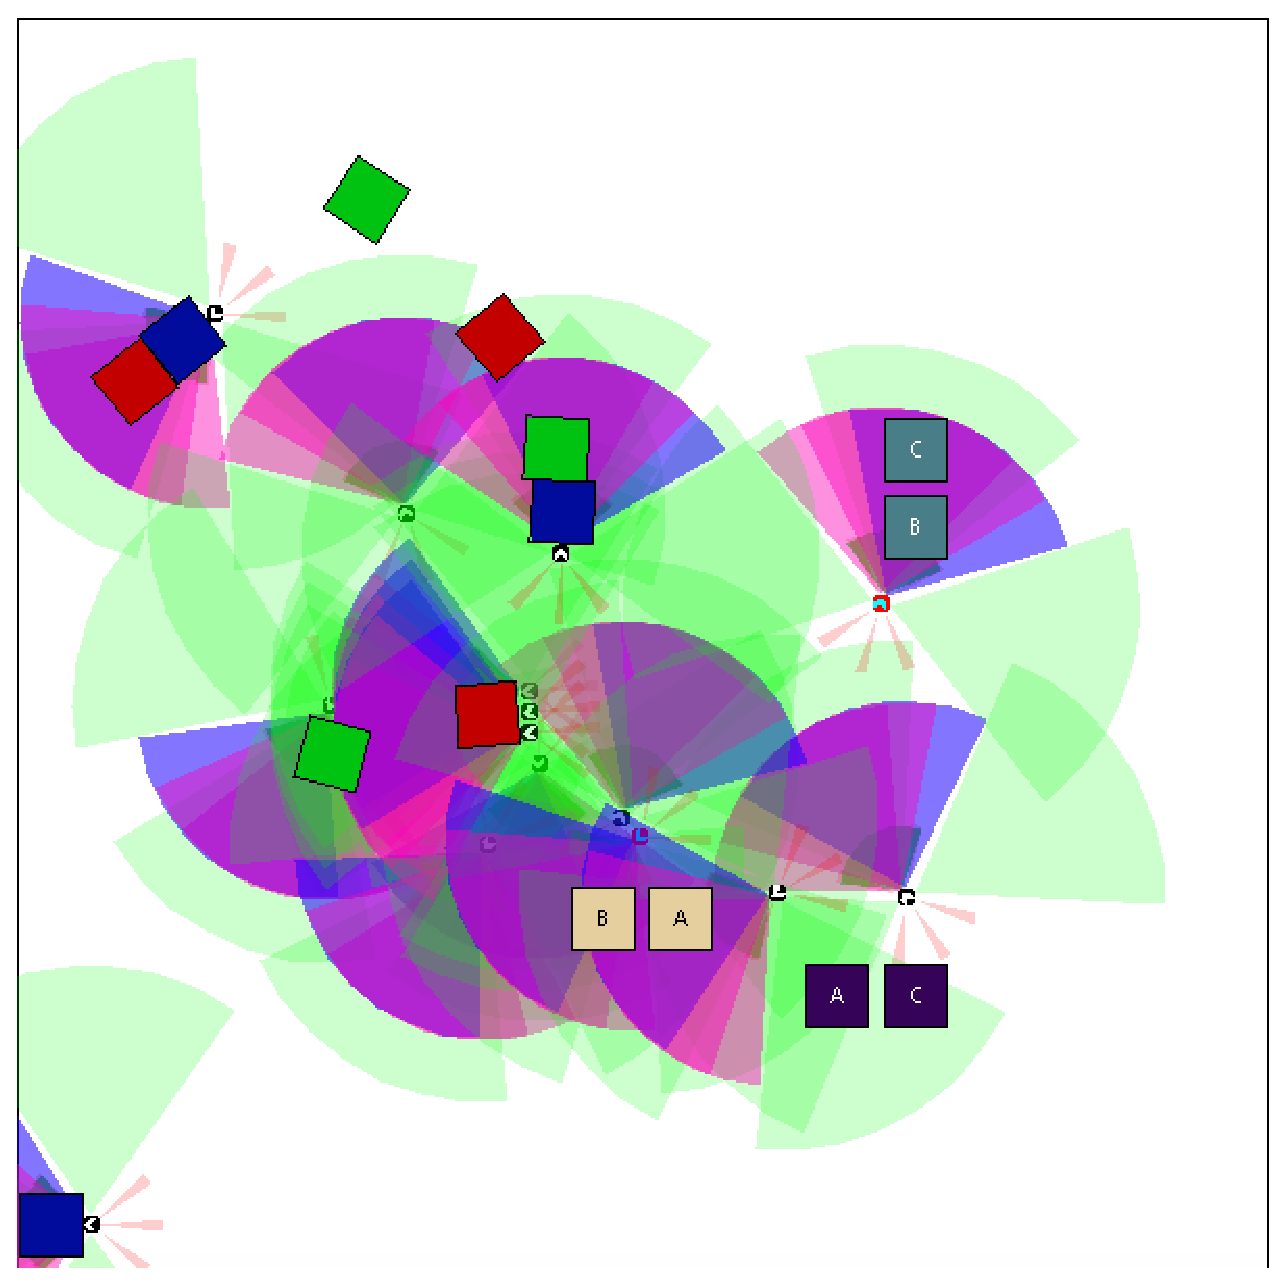
\includegraphics[width=0.40\textwidth]{TaskEnv.eps}
	\caption{Example of the simulation environment.  Robots search for randomly distributed
		type A, B, and C blocks (blue, green and red, respectively).  Other colored and labeled
		blocks indicate those already connected in construction zones.
		Different coloured semi-circles emanating from each
		robot represent the field of view of currently active different sensor types (table \ref{tab:simParameters}).}\label{fig:taskEnv}
\end{figure}


\begin{figure}[t]
	\centering
	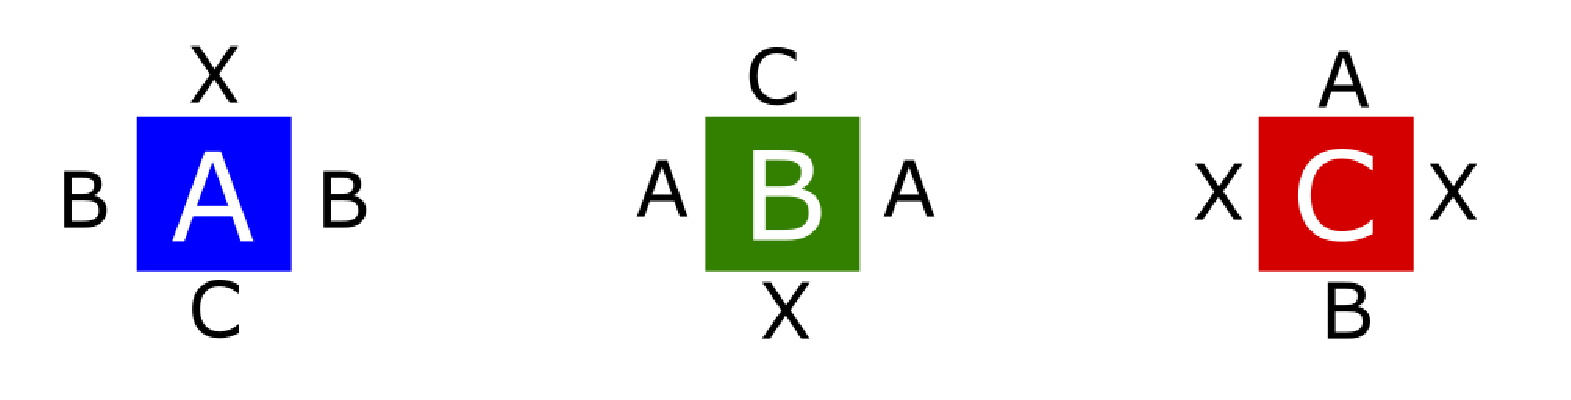
\includegraphics[width=0.5\textwidth]{ConstructionSchema.eps}
	\caption{Task level 3 construction schema: \textit{A}, \textit{B}, and \textit{C} are the block types.  The label on
		each side of each block type indicates what block type can be connected to this side.  An \textit{X} label indicates
		that no block can be connected.}\label{fig:constructionSchema}
\end{figure}

\subsection{Collective Construction Task}\label{subsec:constructionTask}
This task required the robot team to search the environment for building-blocks and
cooperatively push them together in order that they connected to form a structure,
where connected blocks then formed a construction zone.
Task complexity was equated with the degree of cooperation required to collectively
push blocks and connect them together in the construction zone \hl{and whether or not
a construction schema was required. CAN JUST TAKE THIS LAST BIT OUT?}
In this construction task, there were three block types, \textit{A}, \textit{B} and \textit{C}
requiring one, two and three robots to push, respectively. \hl{MENTION THAT THE RESPECTIVE BLOCK TYPES ARE ONLY PRESENT IN EACH OF THE RESPECTIVE LEVELS, RESPECTIVELY}
Cooperation occurred when at least two robots simultaneously pushed a type \textit{B} block,
or at least three robots pushed a type \textit{C} block. \hl{THEREFORE THE FIRST DIFFICULTY LEVEL REQUIRES NO COOPERATION BETWEEN THE ROBOTS}

Table \ref{tab:taskComplexity} presents the three levels of difficulty for the
collective construction task.  Level $1$ was the least complex as it did not require
any cooperation, given that it in this case there were only type \textit{A}
blocks in the environment.
\hl{Level $2$ was of medium complexity as there are equal numbers of type \textit{A},
\textit{B}, and \textit{C} blocks in the environment, where block types \textit{B} and \textit{C} required
at least two and three robots to push, respectively. LEVEL 2 IS OF MEDIUM COMPLEXITY BECAUSE THERE ARE ONLY TYPE B BLOCKS PRESENT IN THE ENVIRONMENT, REQUIRING ONLY 2 ROBOTS TO MOVE A SINGLE BLOCK.}
Level $3$ was the most complex, as it required the same degree of cooperation as task level
$2$, though blocks had to be connected according to a construction schema. \hl{LEVEL 3 IS THE MOST COMPLEX/DIFFICULT AS IT CONSISTED OF ONLY TYPE C BLOCKS IN THE ENVIRONMENT WHICH REQUIRE 3 ROBOTS TO MOVE A SINGLE BLOCK THUS EQUATING TO THE HIGHEST DEGREE OF COOPERATION REQUIRED.}

Figure \ref{fig:constructionSchema}
illustrates this construction schema, where the label on each of the
four sides of each block type indicates what other block type can be connected to the given side.

\hl{should this part just be removed since there is no longer a construction schema being used? or should I add a new construction schema image showing that there is only one type of resource in each level and that they can be connected on any side of each other.}

The \textit{X} label indicates that no block can be connected to a given side.

The construction zone was formed via at least two blocks pushed together and
was thus any structure being built in the environment.
Once a construction zone was created, all blocks attached to it were fixed in position
and could not be disconnected.
The task mandated a maximum of three construction zones and unconnected blocks
had to be pushed and connected to one of these construction zones.

For each difficulty level of the task, a different type of resource block is implemented (as shown in table \ref{tab:taskComplexity}) in order to control the level of cooperation required in the task.

Team task performance was calculated as the number of blocks connected in construction zones
during a team's lifetime (equation \ref{equ:FitnessFunction}),
where average task performance was calculated as the highest task
performance selected at the end of each run ($100$ generations) and averaged over $20$ runs
(table \ref{tab:simParameters}).


The fitness function to direct controller evolution was a weighted sum of
the number of times \textit{type A} blocks were pushed by \textit{one robot}
and connected (\(a\) in equation \ref{equ:FitnessFunction}), the number of times \textit{type B} blocks were pushed
by \textit{two robots} and connected (\(b\) in equation \ref{equ:FitnessFunction}),
and the number of times \textit{type C} blocks were pushed by \textit{three robots}
and connected (\(c\) in equation \ref{equ:FitnessFunction}).

\begin{equation}\label{equ:FitnessFunction}
f = r_a a + r_b b + r_c c
\end{equation}

Parameter tuning experiments found that setting the weights (reward values \(r_a\), \(r_b\) and \(r_c\))
in equation \ref{equ:FitnessFunction} to 0.3, 0.6, and 1.0, respectively, resulted in functional controller evolution.
Fitness was normalized to the range \([0.0, 1.0]\) using the maximum possible fitness yielded from
all blocks being pushed and connected in construction zones.
%\hlcyan{this is the new content}
%Fitness was normalized to the range \([0.0, 1.0]\) using the total number of each type of block present in the task scenario.

\begin{table}
	\renewcommand{\arraystretch}{1.30}
	\caption{Experiment, Neuro-evolution and Sensor Parameters}\label{tab:simParameters}
	\centering
	\begin{tabular}{llc}
		\hline
		Generations	                                           & 100	\\
		Sensors per robot                                      & 11, 8, 4 \\	
		Evaluations per genotype                               & 3  \\
		Experiment runs                                        & 20 \\
		Environment length, width                              & 20 \\
		Max Distance (Robot movement per iteration)            & 1.0 \\
		Team size                                              & 15 \\
		Team Lifetime (Simulation iterations)                  & 1000 \\	
		Lifetimes per generation                               & 3 \\
		Type A blocks (1 robot to push)                        & 15 \\
		Type B blocks (2 robots to push)                       & 15 \\
		Type C blocks (3 robots to push)                       & 15 \\
		\hline
		\multirow{4}{*}{Mutation rate} & Add neuron            & 0.25 \\
		& Add connection                                       & 0.008  \\
		& Remove connection                                    & 0.002 \\
		& Weight                                               & 0.1  \\
		Population size                                        & 150 \\
		Survival rate                                          & 0.3 \\
		Crossover proportion                                   & 0.5 \\
		Elitism proportion                                     & 0.1 \\
		CPPN topology                                          & Feed-forward           \\
		CPPN inputs                                            & Position, delta, angle \\
		\hline
		Sensor                                                 & Range     & FOV \\
		\hline
		Proximity Sensor		                               & 	1.0	   &  0.2  \\
		Ultrasonic Sensor		                               &	4.0    &  1.2  \\
		Ranged Colour Sensor	                               &	3.0	   &  1.5 \\
		Low-Res Camera			                               & 	3.0	   &  1.5 \\
		Colour Proximity Sensor                                & 	3.0	   &  3.0 \\
		\hline
	\end{tabular}
\end{table}

\begin{table}[t]
	\renewcommand{\arraystretch}{1.30}
	\caption{Task Complexity.}\label{tab:taskComplexity}
	\centering
	\begin{tabular}{lccc}
		\hline
		Construction Task Complexity                               & Level 1     & Level 2    & Level 3   \\
		\hline
		Type A blocks (1 robot to push)	                           & 	15	     & 0          & 0  \\
		Type B blocks (2 robots to push)		                   &	0 	     & 15         & 0  \\
		Type C blocks (3 robots to push)	                       &  	0	     & 0          & 15  \\
		\hline
	\end{tabular}
\end{table}

\subsection{Experiment Design}\label{subsec:expDesign}

Experiments evaluated the \textit{morphological robustness} of HyperNEAT evolved controllers for
robot teams that must accomplish collective construction tasks of increasing \hl{of increasing degrees of cooperation/difficulty}
complexity (section \ref{subsec:constructionTask}).
We measured the average comparative task performance of controllers evolved
for a given team morphology and task complexity \hl{difficulty?} where such controllers were
then transferred to
and re-evaluated in other team morphologies.
Thus, teams that achieved an average task performance that was not significantly lower
across all \textit{re-evaluated} morphologies were considered to be \textit{morphologically robust}.

This study comprised of three experiment sets where a single set consisted of evolving a controller for a given team morphology $1-3$ (table \ref{tab:morphConfigs}) for three levels of increasing task complexity, requiring increasing levels of cooperation (table \ref{tab:taskComplexity})

Each experiment set comprised a controller evolution stage and a re-evaluation stage
(morphological robustness test).
For controller evolution, each experiment applied HyperNEAT to evolve team behavior for
$15$ robots for $100$ generations,
where a generation comprised \hl{three} team \textit{lifetimes} ($1000$ simulation iterations).
Each team lifetime tested different robot starting positions, orientations, and block locations
in the simulation environment.
The fittest controller evolved for each task level (yielding the highest absolute task performance)
was then \textit{re-evaluated} for morphological robustness in all other morphologies.
For example, the fittest controller evolved for morphology $1$ was re-evaluated in morphologies
$2$ and $3$ and the average task performance calculated across all re-evaluation runs.
%($1$ to $7$ in table \ref{tab:morphConfigs}) for the given task.

Each re-evaluation run was \textit{non-evolutionary}, where controllers were not further evolved,
and each re-evaluation run was equivalent to one team lifetime.
Re-evaluation runs were repeated $20$ times for a given morphology, in order to account for random variations in robot and block
starting positions and orientations.
For each fittest controller, re-evaluated in a given morphology, an average task performance was
calculated over these $20$ runs, and then an overall average task performance was computed for
all re-evaluated morphologies.

As per this study's objectives, these morphological re-evaluation
runs tested how robust the fittest evolved controllers (for a given morphology) were to variations
in that morphology.
Thus, re-evaluating the fittest controllers on other morphologies emulated sensor loss due
to damage or new robot morphologies introduced due to changing task constraints.

\begin{figure*}[t]
	\begin{minipage}{0.5\textwidth}
		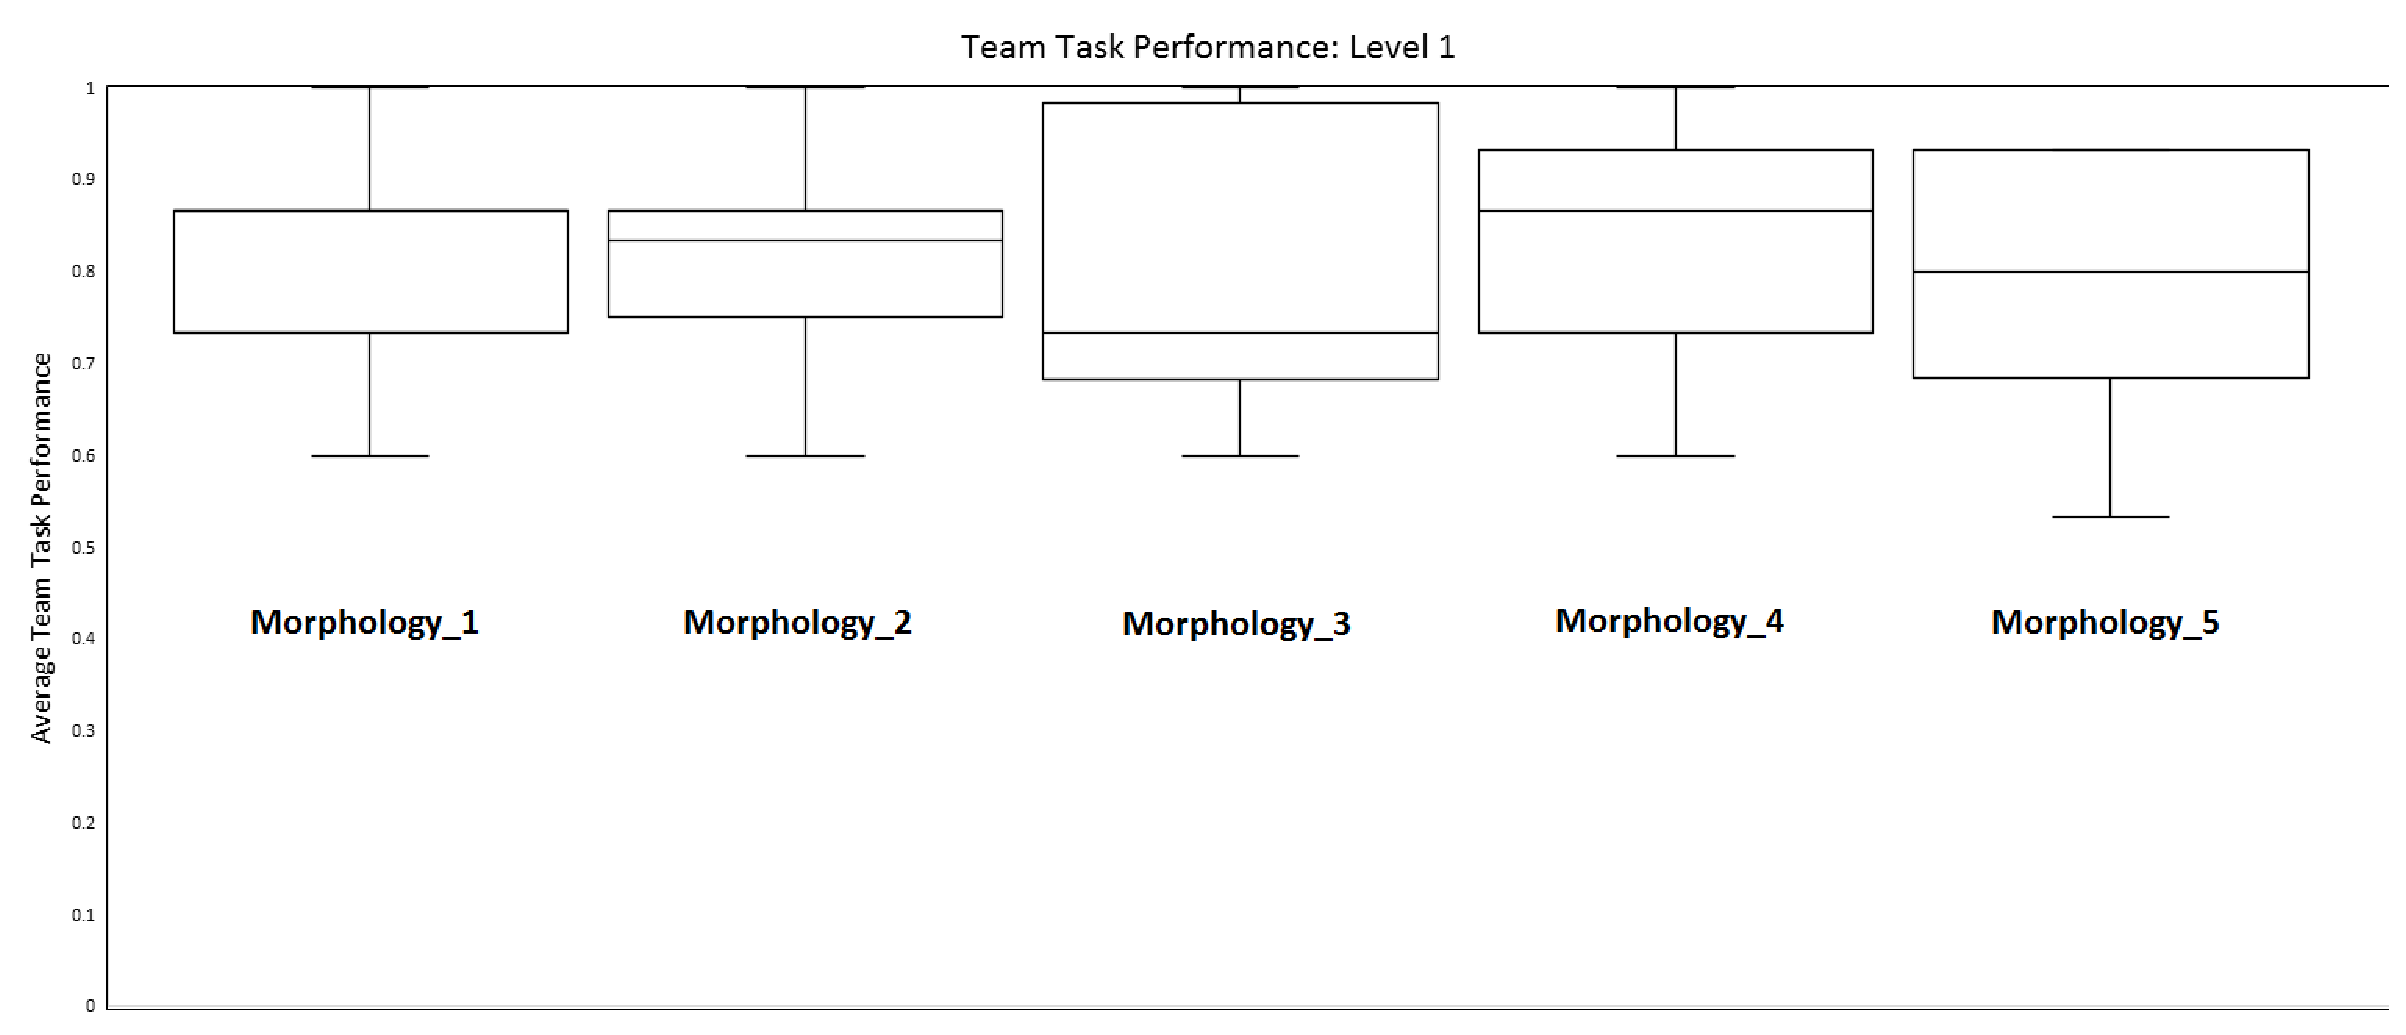
\includegraphics[width=\textwidth]{Evo_BoxPlot_Level1.eps}
	\end{minipage}
	\begin{minipage}{0.5\textwidth}
		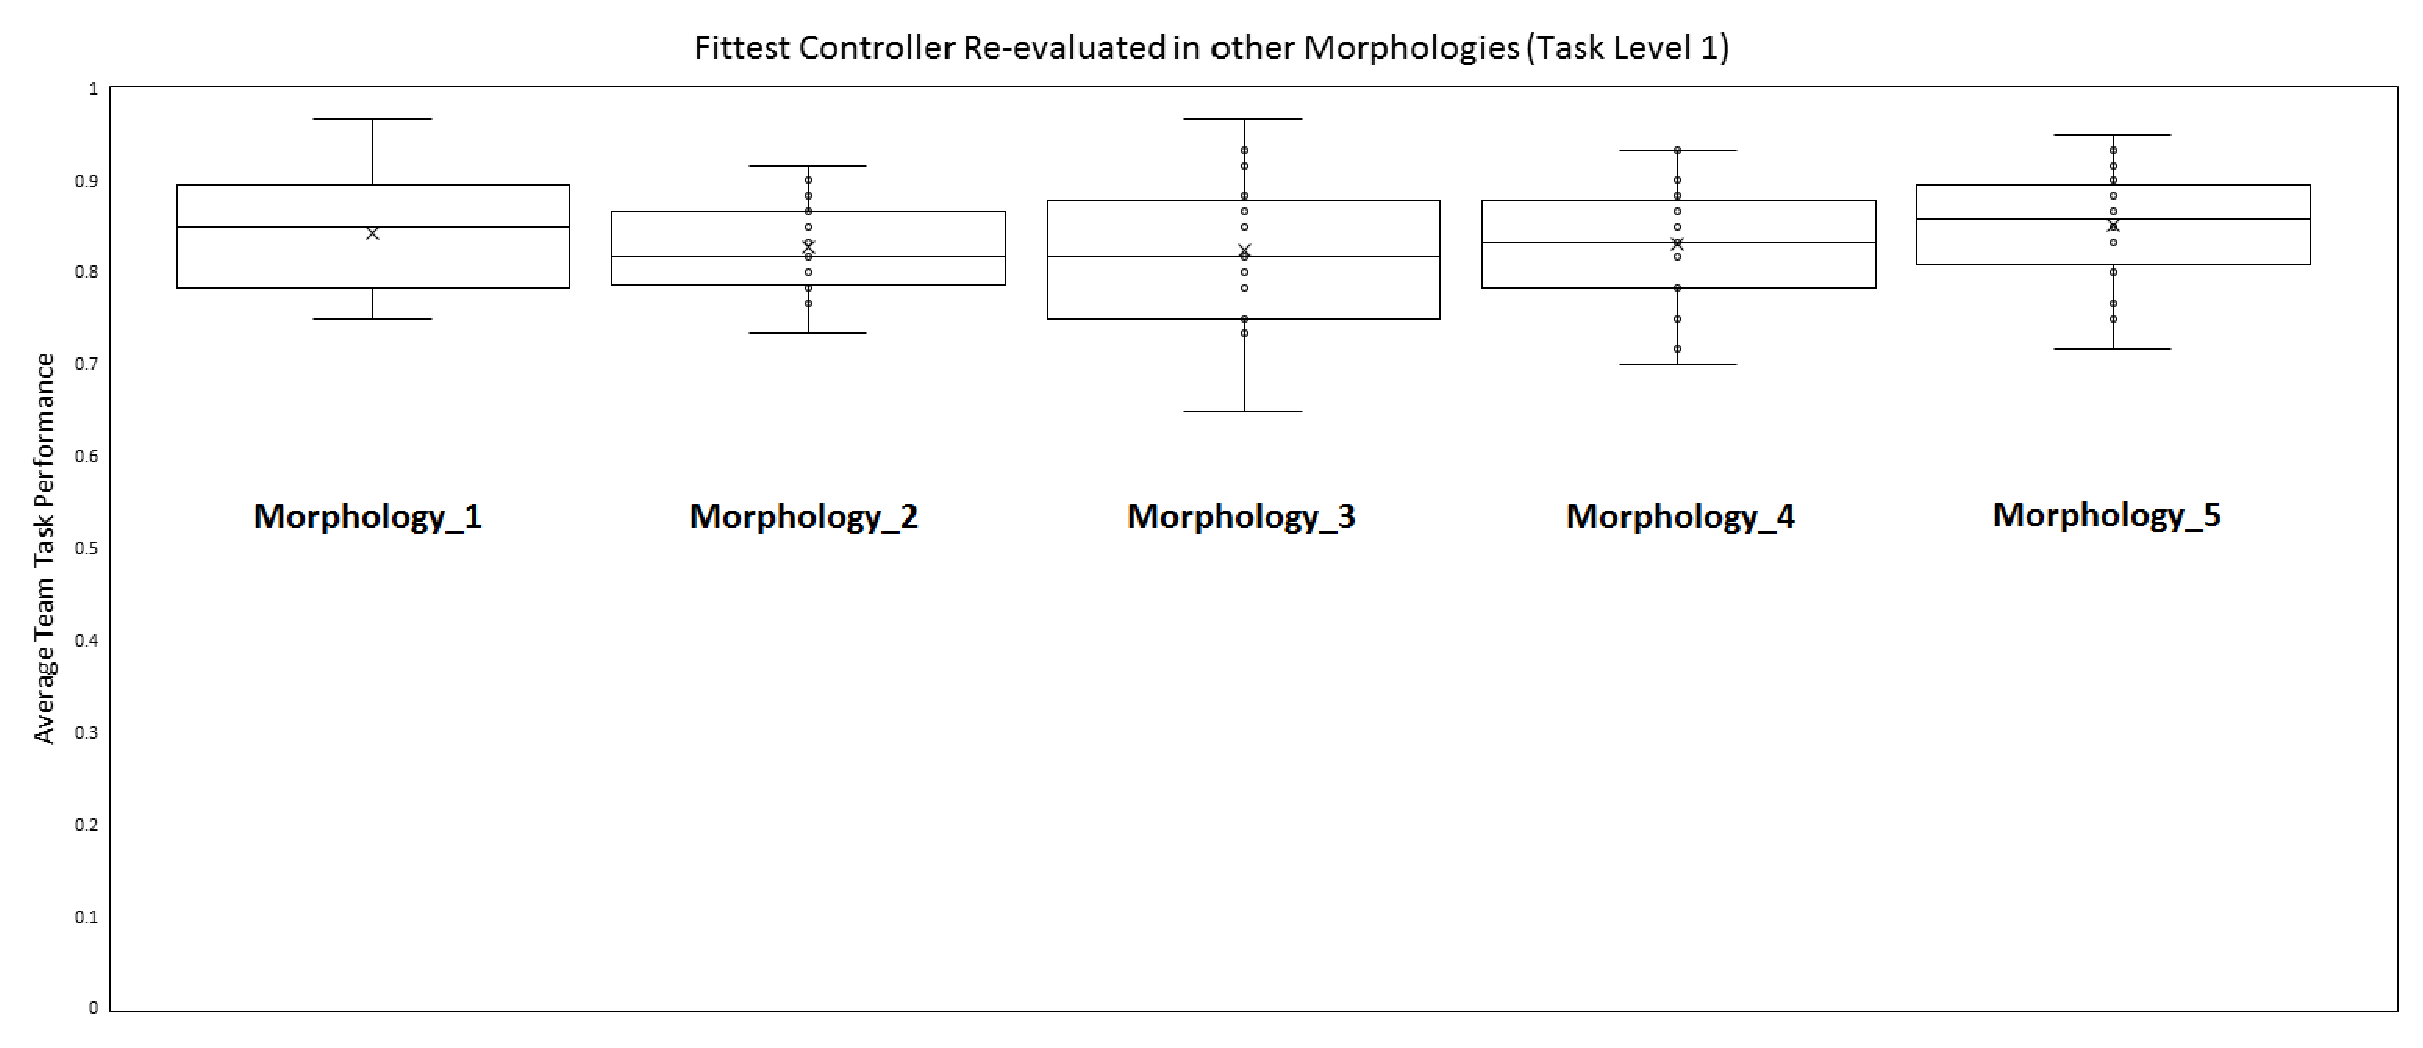
\includegraphics[width=\textwidth]{Level1_ReEval.eps}
	\end{minipage}
	\caption{\textit{Left column:} Average team task performance for controller evolution (\textit{task level 1})
		given morphologies $1-5$ (depicted from left to right).
		\textit{Right column:} Average task performance given the fittest controller evolved
		for each successive morphology ($1-5$, shown left to right) re-evaluated in all other morphologies.
		For example: Left-most plot is average task performance of fittest controller evolved for
		morphology $1$, re-evaluated in morphologies $2-5$.  Right-most plot is the average task performance
		of fittest controller evolved for morphology $5$, re-evaluated in morphologies $1-4$.}\label{fig:level1results}
\end{figure*}

\begin{figure*}[t]
	\begin{minipage}{0.5\textwidth}
		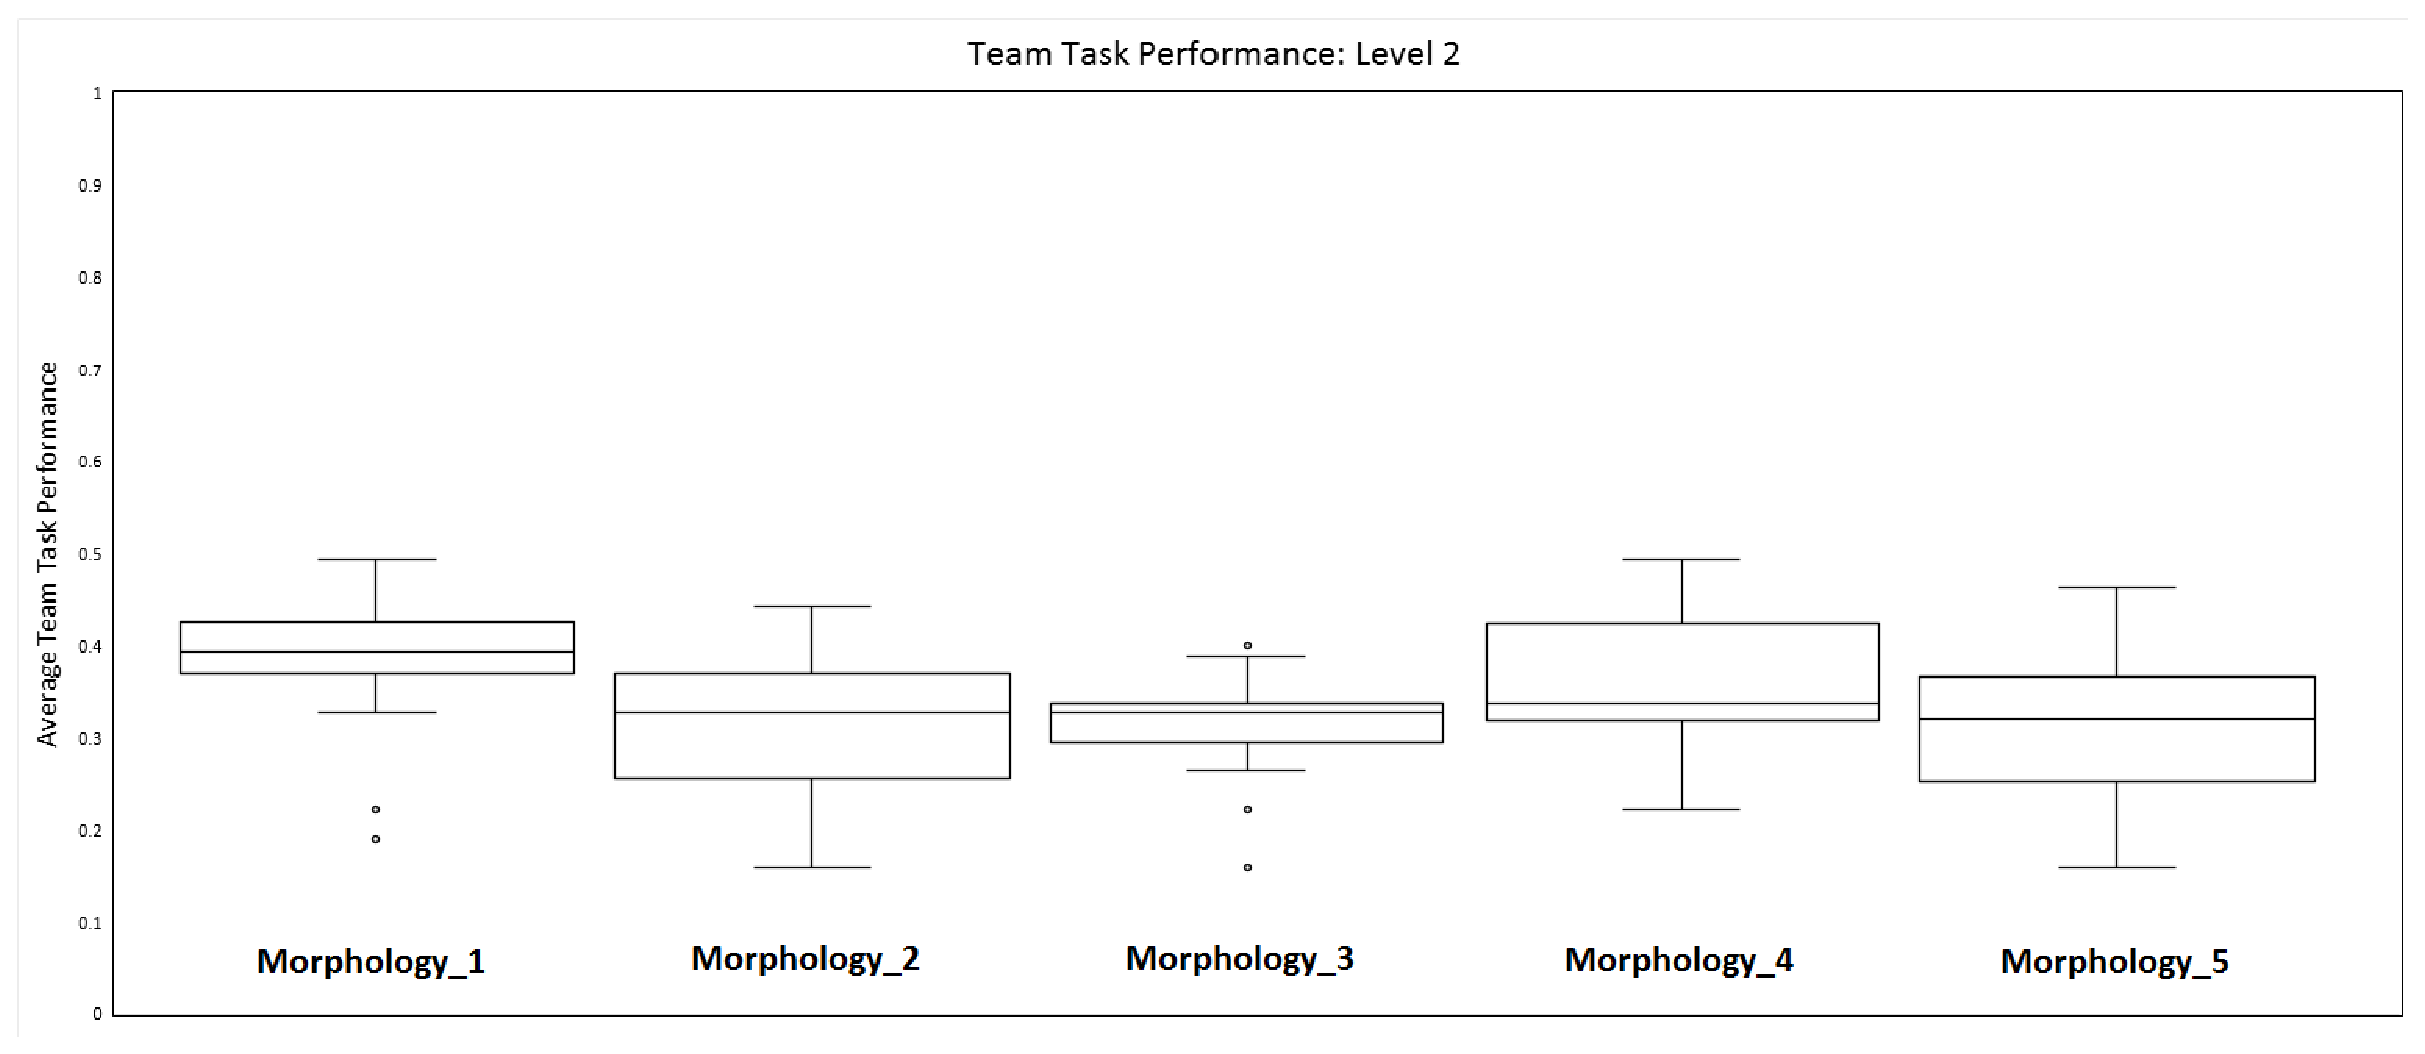
\includegraphics[width=\textwidth]{Evo_BoxPlot_Level2.eps}
	\end{minipage}
	\begin{minipage}{0.5\textwidth}
		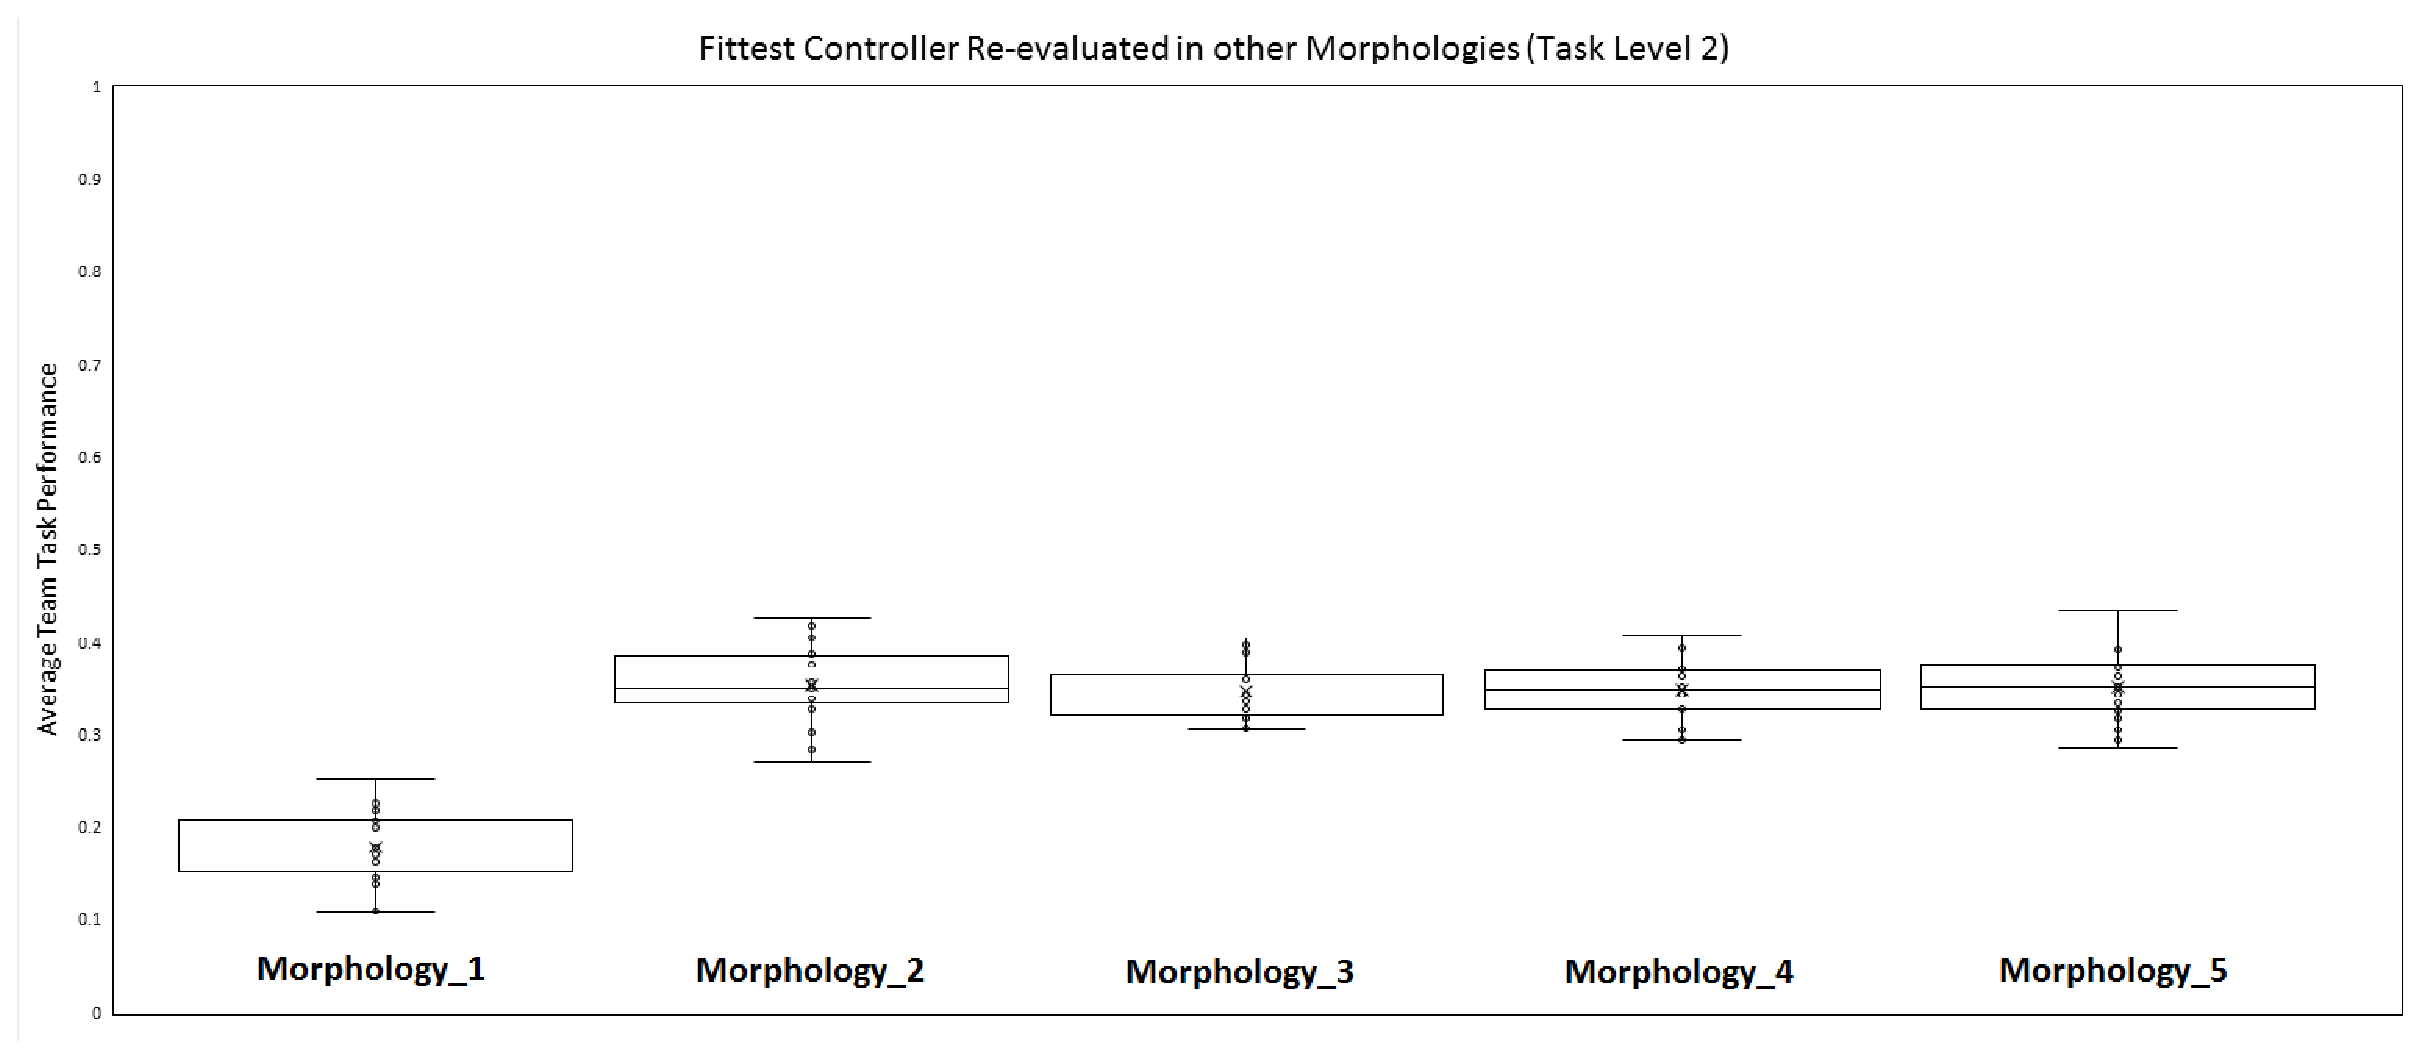
\includegraphics[width=\textwidth]{Level2_ReEval.eps}
	\end{minipage}
	\caption{\textit{Left column:} Average team task performance for controller evolution (\textit{task level 1})
		given morphologies $1-5$ (depicted from left to right).
		\textit{Right column:} Average task performance given the fittest controller evolved
		for each successive morphology ($1-5$, shown left to right) re-evaluated in all other morphologies.
		For example: Left-most plot is average task performance of fittest controller evolved for
		morphology $1$, re-evaluated in morphologies $2-5$.  Right-most plot is the average task performance
		of fittest controller evolved for morphology $5$, re-evaluated in morphologies $1-4$.}\label{fig:level2results}
\end{figure*}

\begin{figure*}[t]
	\begin{minipage}{0.5\textwidth}
		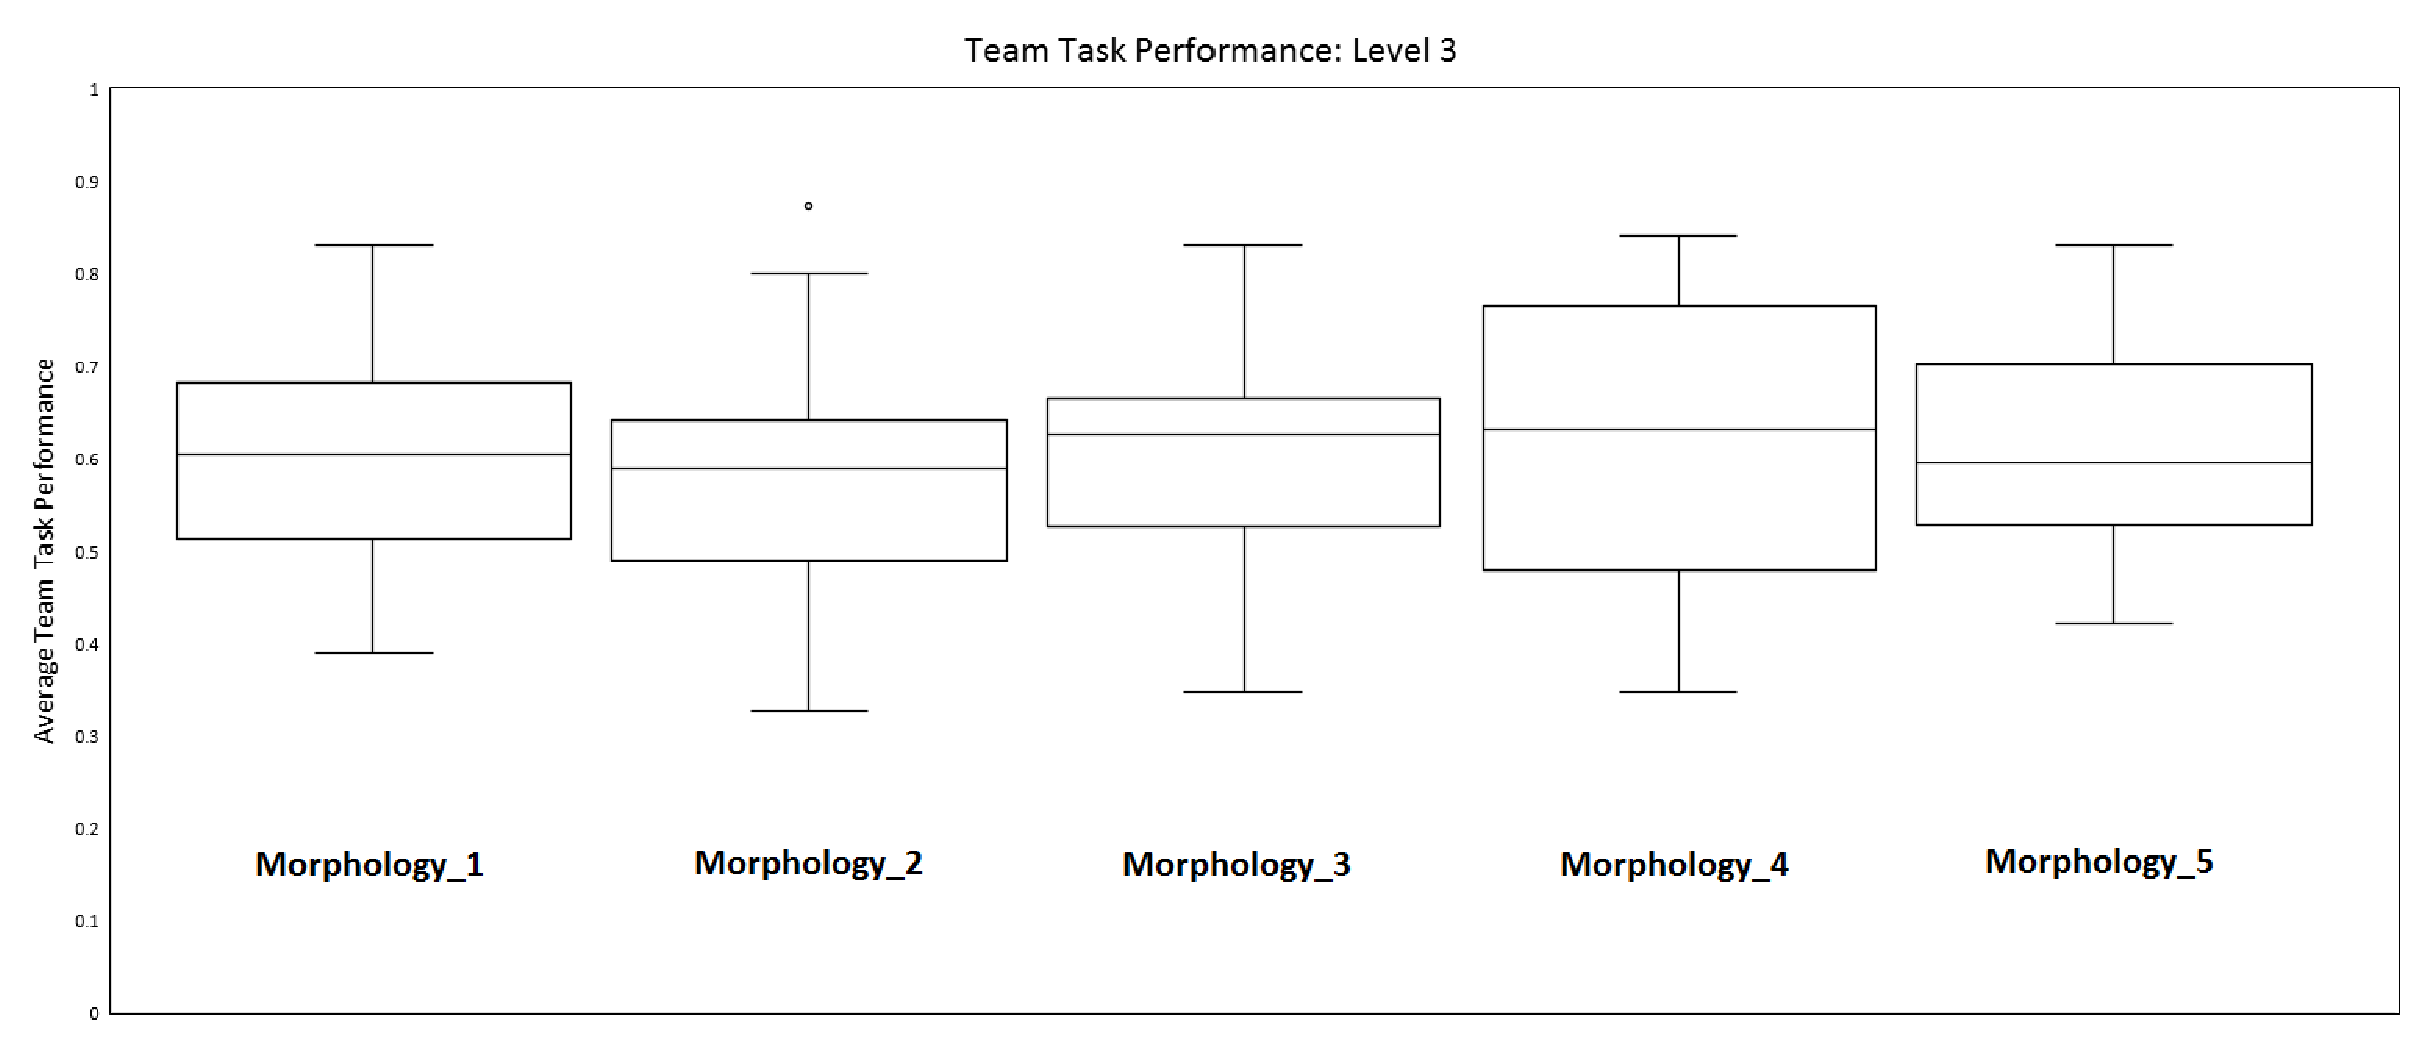
\includegraphics[width=\textwidth]{Evo_BoxPlot_Level3.eps}
	\end{minipage}
	\begin{minipage}{0.5\textwidth}
		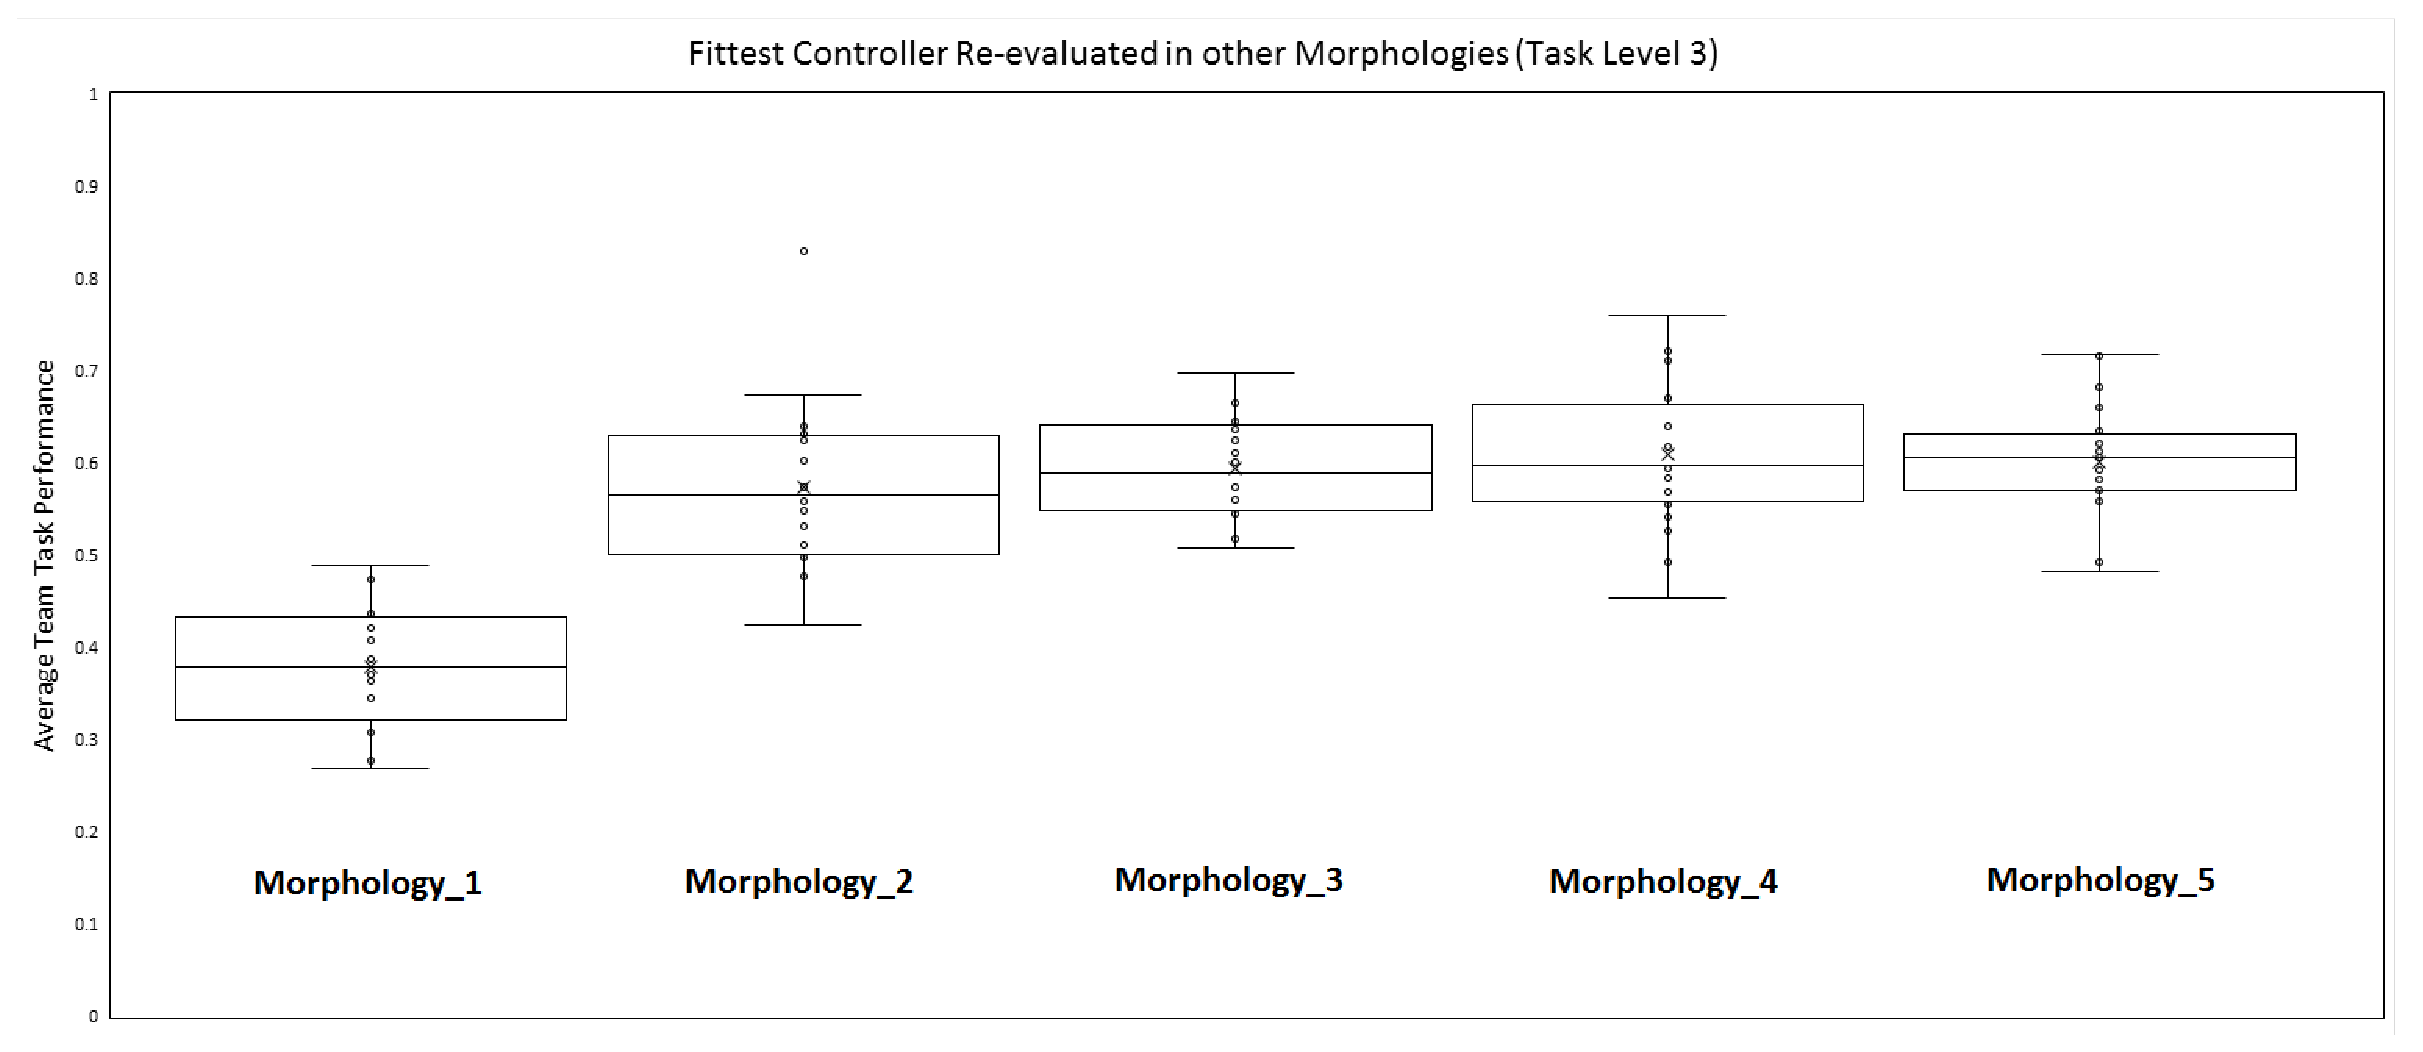
\includegraphics[width=\textwidth]{Level3_ReEval.eps}
	\end{minipage}
	\caption{\textit{Left column:} Average team task performance for controller evolution (\textit{task level 1})
		given morphologies $1-5$ (depicted from left to right).
		\textit{Right column:} Average task performance given the fittest controller evolved
		for each successive morphology ($1-5$, shown left to right) re-evaluated in all other morphologies.
		For example: Left-most plot is average task performance of fittest controller evolved for
		morphology $1$, re-evaluated in morphologies $2-5$.  Right-most plot is the average task performance
		of fittest controller evolved for morphology $5$, re-evaluated in morphologies $1-4$.}\label{fig:level3results}
\end{figure*}

\appendix
%Appendix A
\section{Headings in Appendices}
The rules about hierarchical headings discussed above for
the body of the article are different in the appendices.
In the \textbf{appendix} environment, the command
\textbf{section} is used to
indicate the start of each Appendix, with alphabetic order
designation (i.e., the first is A, the second B, etc.) and
a title (if you include one).  So, if you need
hierarchical structure
\textit{within} an Appendix, start with \textbf{subsection} as the
highest level. Here is an outline of the body of this
document in Appendix-appropriate form:
\subsection{Introduction}
\subsection{The Body of the Paper}
\subsubsection{Type Changes and  Special Characters}
\subsubsection{Math Equations}
\paragraph{Inline (In-text) Equations}
\paragraph{Display Equations}
\subsubsection{Citations}
\subsubsection{Tables}
\subsubsection{Figures}
\subsubsection{Theorem-like Constructs}
\subsubsection*{A Caveat for the \TeX\ Expert}
\subsection{Conclusions}
\subsection{References}
Generated by bibtex from your \texttt{.bib} file.  Run latex,
then bibtex, then latex twice (to resolve references)
to create the \texttt{.bbl} file.  Insert that \texttt{.bbl}
file into the \texttt{.tex} source file and comment out
the command \texttt{{\char'134}thebibliography}.
% This next section command marks the start of
% Appendix B, and does not continue the present hierarchy
\section{More Help for the Hardy}

Of course, reading the source code is always useful.  The file
\path{acmart.pdf} contains both the user guide and the commented
code.

\begin{acks}
  The authors would like to thank Dr. Yuhua Li for providing the
  matlab code of  the \textit{BEPS} method. 

  The authors would also like to thank the anonymous referees for
  their valuable comments and helpful suggestions. The work is
  supported by the \grantsponsor{GS501100001809}{National Natural
    Science Foundation of
    China}{http://dx.doi.org/10.13039/501100001809} under Grant
  No.:~\grantnum{GS501100001809}{61273304}
  and~\grantnum[http://www.nnsf.cn/youngscientsts]{GS501100001809}{Young
    Scientsts' Support Program}.

\end{acks}
